\chapter{The implementation of phonic voicing contrast in children’s speech: some explorations of clinical data}\label{ch:zuleicacamarg13}
\chapterauthor[1]{Fabiana Nogueira Gregio}
\chapterauthor[1]{Zuleica Camargo}
\begin{affils}
\chapteraffil[1]{Pontifícia Universidade Católica de São Paulo}
\end{affils}


%%%%%%%%%%%%%%%%%%%%%%%%%%%%%%%%%%%%%%%%%%%%%%%%%%%%%%%%%%%%%%%%%%%%%%
\begin{abstract}
The objective was to investigate the implementation strategies of phonic
voicing contrast in Brazilian Portuguese in a group of children with speech
disorders in comparison to a control group. From the production of target words
with unvoiced and voiced plosive sounds, in contexts of tonic and post-tonic
syllables, a set of acoustic measures was extracted and analyzed, a perception
experiment was applied, and the acoustic and auditory spheres were explored by
means of statistical analysis. The investigation showed that the subjects
performed intermediate productions towards the determinant characteristics of
the voicing contrast. More than one acoustic cue was implemented for auditory
judgment of the voicing contrast.
\end{abstract}


\section{Introduction}
Speech disorders trigger continual investigations into the refined mechanisms
of speech. Among the complaints of speech disorders, the speech therapy
clinical setting is faced with the demand to care for cases of
“absence/exchange of voiced sounds” \citep{keskesoares2004,mota2012}.
In traditional phonological views, such disorder is regarded as the
absence or substitution of phonemes or distinctive features. However, clinical
evaluations supported by acoustic-phonetic analyses have shown the presence of
acoustic cues indicative of the realization of the sound considered absent.

Studies suggest that speakers mark a phonic distinction potentially perceived
by them and revealed through intermediate rather than categorical productions,
yet not always identified by the listener \citep{levy1993,ficker2003,gregio2005,rodrigues2008,gregio2011,pereira2012}.

These productions can be investigated if enlightened by speech production and
perception theoretical models that contemplate the dynamic and gradient
character of speech, fundamentally relying on the use of speech analysis
instruments for explanation \citep{silva2001,gregio2011,albano2007,silva2010}.

Regarding the plosive obstruent consonants of Brazilian Portuguese (BP), the
unvoiced-voiced pairs [p]-[b], [t]-[d], and [k]-[g] constitute the repertoire
of sounds, characterized by the respective places of articulation bilabial,
dental, and velar \citep{silva2001,camargo2008}.

Physiologically, the voicing production in plosives involves fine motor
coordination of glottic (vocal fold vibration) and supraglottic (vocal tract
obstruction) movements \citep{sweeting_voice_1982,shimizu1996,gregio2005}.
Integrity of lung volume, aerodynamic conditions of the glottis,
laryngeal muscles, phono-articulatory organs, and auditory system are required
\citep{hoit1993,shimizu1996,hoole1999}.

Acoustically, the production of unvoiced plosives involves the generation of a
transient noise source, the acoustic result of complete constriction at some
point in the vocal tract followed by its release. In voiced plosives, there are
two sound sources: the transient noise coupled with the voice source resulting
from the vibration of the vocal folds \citep{kent1992,johnson2003}.

One of the acoustic measures used and studied in the investigation of voicing
contrasts is voice-onset-time (VOT) \citep{lisker1964,behlau,kent1992,levy1993,shimizu1996,cho1999,camargo2000,rocca2003}.
Other acoustic measures
have been reported in voicing contrast studies, such as consonant duration,
duration of vowels adjacent to the consonant, fundamental frequency (f0) at the
beginning of the vowel following the consonant, frequency of the first formant
(F1) at the beginning of the vowel following the consonant, and burst 
\citep{barton1980,shimizu1996,veloso1997,van_alphen2004,benki2005,lousada2005,barroco_2007,whalen2007,morris2008,hanson2009,tachibana2012}.

In the BP literature, especially in the clinical context, VOT is still
highlighted in the voicing contrast. Studies on this issue in various speech
situations suggest that more than one acoustic cue seems to be involved
\citep{behlau,levy1993,barbosa1996,madureira,ficker2003,gregio2005,gurgueira2006,barzaghi2007,bonatto2007,britto2010,gregio2011,schliemann2011,souza2010,berti2012,melo2012,pereira2012}.

Thus, the objective of this study was to investigate the implementation
strategies of phonic voicing contrast in BP in a group of children with speech
disorders in comparison to a control group.

%%%%%%%%%%%%%%%%%%%%%%%%%%%%%%%%%%%%%%%%%%%%%%%%%%%%%%%%%%%%%%%%%%%%%%
\section{Methods}
Six subjects aged between 7 and 10 years old participated in this study, two
females and four males, of whom three had a diagnosis of speech disorders
related to voicing contrast (studied group) and three had no speech disorders
(control group).

The selected subjects presented audiological evaluation with normal hearing
thresholds, had a negative history of neurological, voice disorders and other
speech disorders unrelated to voicing contrast, and were BP speakers with no
reference to bilingualism.

The age group did not include the voice change phase, which could have affected
the voice source as a result of physiological changes in the vocal tract
\citep{behlau1995}. Within the established age limits, differences in
laryngeal acoustic measures were not significant between male and female
children \citep{andrade2009}.

The subjects participated in the speech production data collection, carried out
in a speech laboratory. The corpus consisted of recordings of the subjects
reading, with five repetitions in random order, sentences following the
syllabic structure C1V1C2V2 (consonant1-vowel1-consonant2-vowel2). The target
words contained the unvoiced and voiced plosive sounds of BP (papa, baba, tata,
dada, caca, gaga), inserted in the carrier-sentence “Diga
\underline{\hspace{4ex}} baixinho”.

The subjects presented different speech productions regarding the stress of the
target word. Despite the proposed paroxytone stress pattern (for example,
“PApa”), as it is considered the most common in BP, some children produced an
oxytone stress pattern (“paPA”). Thus, the second syllable of the target word
was performed as stressed and post-tonic. To guarantee the reliability of the
data, with the subject maintaining the same stress of the word throughout its
repetitions, the collected corpus was explored through statistical treatment in
order to define distinct contexts that could interfere with the reading of the
data.

Because the acoustic duration parameter is considered the main correlate of
lexical stress in BP (Barbosa, 1996; Aquino, 1997; Gama-Rossi, 1999), duration
measures of the V1C2V2 segments were extracted. As a result (figure \ref{gregio-fig01}), the
acoustic measures showed 100\% predictive value in segregating these speech
samples into two groups and the most influential variables were duration of C2
and V2, equivalent to the duration of the syllable, finding support in the
literature mentioned.

\begin{figure}
\centering
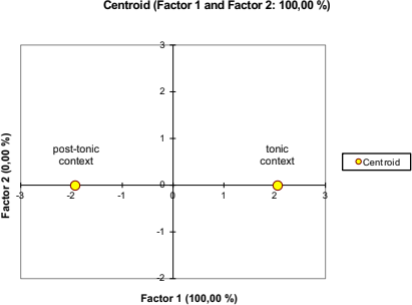
\includegraphics[width=0.7\linewidth]{imgs/gregio-image1.png}
\caption{Centroid graph of the discriminant analysis for estimating the subjects' speech productions in the tonic and post-tonic contexts, based on the extracted acoustic measures.} 
\label{gregio-fig01}
\end{figure}


The speech samples were then classified into studied group and control group
and according to tonic and post-tonic contexts.

The collected data were analyzed acoustically using the PRAAT software and
involved the acoustic inspection of the waveform and broadband spectrogram, and
extraction of the measurements: f0 at the beginning of vowel following the
consonant (V2); f0 at the stationary point of V2; F1 at the beginning of V2; F1
at the stationary point of V2; measures of duration of the plosive consonant
(C2), duration of the previous vowel (V1) and of the following vowel (V2) to
the consonant, and duration of the V1C2V2 excerpt of the target word; measures
of duration of the VOT; and duration measures of the voicing bar. The voicing
bar measures were extracted to contemplate gradient productions and included:
duration of the voicing period (voicing bar period in the consonant stretch
before the articulation release); duration of the voiceless period (length of
the stretch in which there is no voicing bar before the articulation is
released); duration of the voicing pre-plosion period (duration of the voicing
bar when it is performed after a period of silence in an excerpt before the
articulation is released); duration of the total pre-plosion period (total
duration of the stretch prior to the release of the articulation, regardless of
whether or not there is a voice bar); plosion duration (burst duration: period
between the starting point of articulation release and the beginning of the
vowel). The relative duration measures of all extracted duration measures
described above were calculated to eliminate influences from the subject's
speech rate. For sequence of analyses, measures of relative duration were used.

The speech production data were submitted to a battery of statistical tests to
consider the existing variants in speech, as proposed in research developed by
the partnership between researchers and professors from LIAAC-PUCSP and the
Actuaries and Quantitative Methods Department-PUCSP.

The collection of speech perception data was carried out through an experiment
elaborated using the PRAAT software. The sound stimuli consisted of the target
words of the carrier sentences of the subjects' speech productions. Although
the analysis and data reading refer to the V1C2V2 excerpt of the target word,
for the experiment, the target word was edited in its entirety (C1V1C2V2) to
avoid the effects of sample editing. The stimuli were presented in random order
to the judges of the perception experiment.

Thirty-nine judges were selected of the same age and level of education,
without hearing and/or speech complaints and with no connections to the fields
of languages and speech-language pathology. The procedure was performed
individually and with the use of headphones, and each judge orthographically
transcribed the word as he or she heard it (word identification).

Next, a statistical analysis was performed to verify the reliability of the
judges' answers, which resulted in the exclusion of four judges (figure 2). To
analyze the data from the perception experiment, the responses of thirty-five
judges were considered.

\begin{figure}
\centering
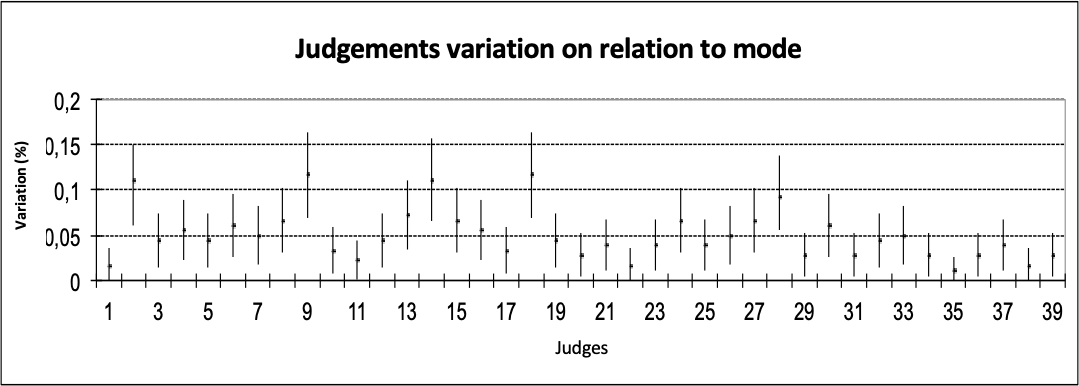
\includegraphics[width=\linewidth]{imgs/gregio-image2.png}
\caption{Representation of the auditory judgment variation of each judge in relation to mode value for verification of the judge's performance.} 
\label{gregio-fig02}
\end{figure}

Based on \citet{johnson2003}, the answers were tabulated in confusion matrices.
Afterwards, the calculation of the auditory distances of the consonant pairs
was performed, allowing visualization in the form of graphs.

After the speech production data and perception experiment data stage, a
logistic regression analysis was performed to explore the acoustic and auditory
spheres. Research was approved by the Ethics Committee, protocol number 119/09.


%%%%%%%%%%%%%%%%%%%%%%%%%%%%%%%%%%%%%%%%%%%%%%%%%%%%%%%%%%%%%%%%%%%%%%
\section{Results and discussion}
Acoustic measures were compared between unvoiced and voiced plosive consonant
pairs and, in general, revealed significant differences and allowed for
classification of the control and studied groups for both stress contexts
(figures \ref{gregio-fig03} and \ref{gregio-fig04}).

\begin{figure}
\centering
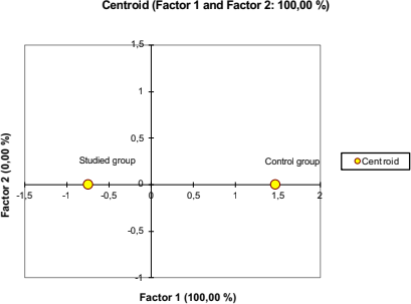
\includegraphics[width=0.7\linewidth]{imgs/gregio-image3.png}
\caption{Centroid graph of the discriminant analysis of the estimation of the group of subjects (studied and control) in the tonic context from the acoustic measures.} 
\label{gregio-fig03}
\end{figure}

\begin{figure}
\centering
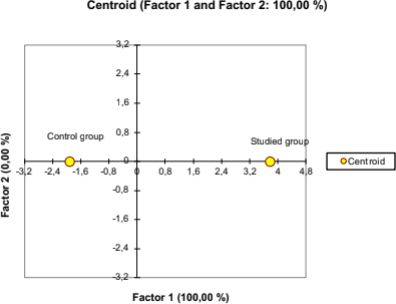
\includegraphics[width=0.7\linewidth]{imgs/gregio-image4.png}
\caption{Centroid graph of the discriminant analysis of the estimation of the group of subjects (studied and control) in the post-tonic context from the acoustic measures.} 
\label{gregio-fig04}
\end{figure}

The results of the calculation of the relative durations of the V1C2V2 excerpt
(figures \ref{gregio-fig05} to \ref{gregio-fig08}), as well as the voicing bar details (figures \ref{gregio-fig09} to \ref{gregio-fig12}), showed
differences between the control and studied groups for both stress contexts.

\begin{figure}
\centering
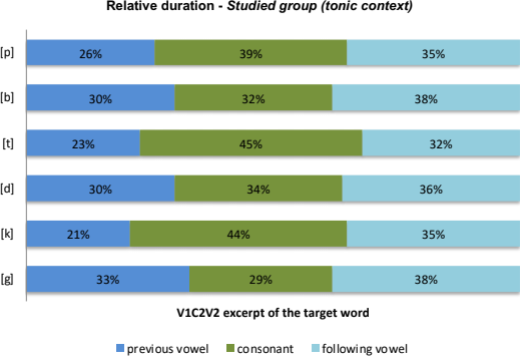
\includegraphics[width=0.9\linewidth]{imgs/gregio-image5.png}
\caption{Schematic representation of the relative duration (\%) of the vowel preceding the consonant, the plosive consonant and the vowel following the consonant, in relation to the V1C2V2 excerpt of the target word, of the speech samples in the tonic context of the studied group.} 
\label{gregio-fig05}
\end{figure}

\begin{figure}
\centering
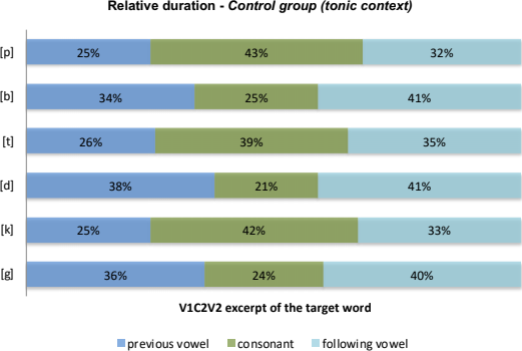
\includegraphics[width=0.9\linewidth]{imgs/gregio-image6.png}
\caption{Schematic representation of the relative duration (\%) of the vowel preceding the consonant, the plosive consonant, and the vowel following the consonant, in relation to the V1C2V2 excerpt of the target word, of the speech samples in the tonic context of the control group.} 
\label{gregio-fig06}
\end{figure}

\begin{figure}
\centering
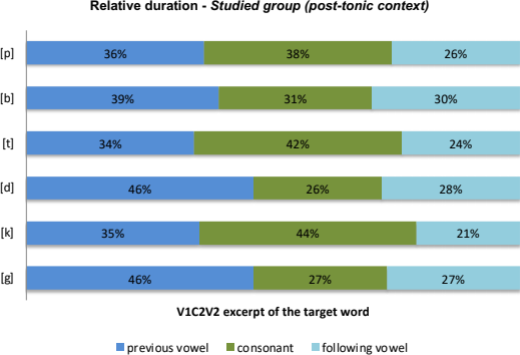
\includegraphics[width=0.9\linewidth]{imgs/gregio-image7.png}
\caption{Schematic representation of the relative duration (\%) of the vowel preceding the consonant, the plosive consonant, and the vowel following the consonant, in relation to the V1C2V2 excerpt of the target word, of the speech samples in the post-tonic context of the studied group.} 
\label{gregio-fig07}
\end{figure}

\begin{figure}
\centering
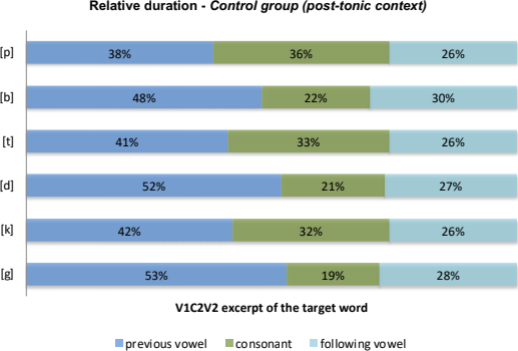
\includegraphics[width=0.9\linewidth]{imgs/gregio-image8.png}
\caption{Schematic representation of the relative duration (\%) of the vowel preceding the consonant, the plosive consonant, and the vowel following the consonant, in relation to the V1C2V2 excerpt of the target word, of the speech samples in the post-tonic context of the control group.} 
\label{gregio-fig08}
\end{figure}

\begin{figure}
\centering
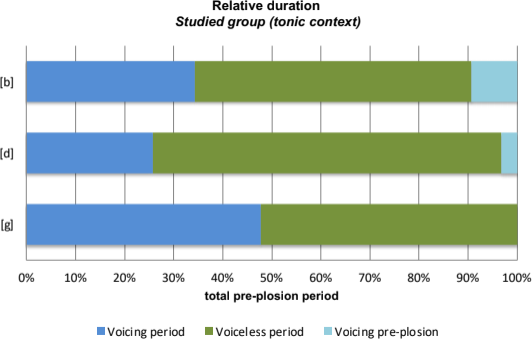
\includegraphics[width=0.9\linewidth]{imgs/gregio-image9.png}
\caption{Schematic representation of the relative duration (\%) of the voicing period, voiceless period, and the voicing pre-plosion period, in relation to the relative duration of the total pre-plosion period, of the speech samples in the tonic context of the studied group.} 
\label{gregio-fig09}
\end{figure}

\begin{figure}
\centering
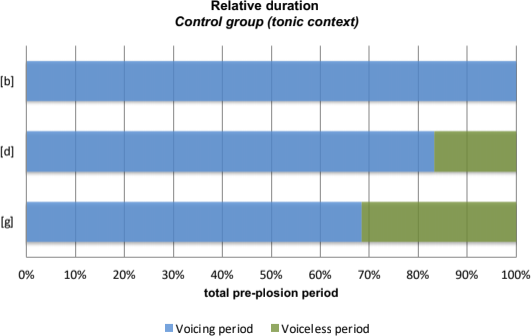
\includegraphics[width=0.9\linewidth]{imgs/gregio-image10.png}
\caption{Schematic representation of the relative duration (\%) of the voicing period and voiceless period, in relation to the relative duration of the total pre-plosion period, of the speech samples in the tonic context of the control group.} 
\label{gregio-fig10}
\end{figure}

\begin{figure}
\centering
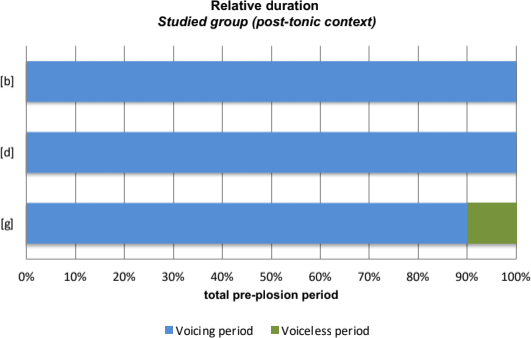
\includegraphics[width=\linewidth]{imgs/gregio-image11.png}
\caption{Schematic representation of the relative duration (\%) of the voicing period and voiceless period, in relation to the relative duration of the total pre-plosion period, of the speech samples in the post-tonic context of the studied group.} 
\label{gregio-fig11}
\end{figure}

\begin{figure}
\centering
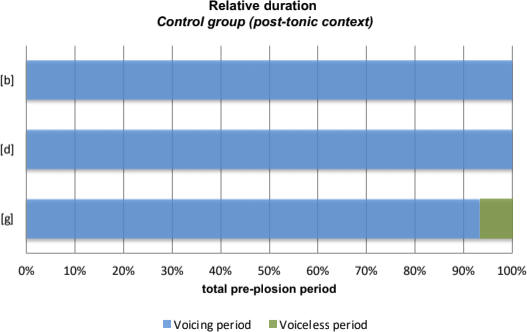
\includegraphics[width=0.9\linewidth]{imgs/gregio-image12.png}
\caption{Schematic representation of the relative duration (\%) of the voicing period and voiceless period, in relation to the relative duration of the total pre-plosion period, of the speech samples in the post-tonic context of the control group.} 
\label{gregio-fig12}
\end{figure}

In terms of perception, auditory distances were smaller for samples from the
studied group compared to the control group in the tonic context (figure \ref{gregio-fig13}).
For the post-tonic context, the auditory distances were similar in both groups
(figure \ref{gregio-fig14}).

\begin{figure}
\centering
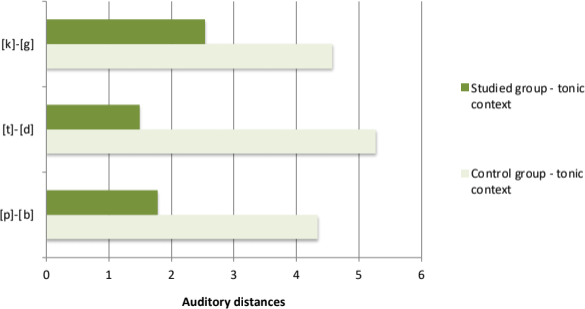
\includegraphics[width=\linewidth]{imgs/gregio-image13.png}
\caption{Auditory distances between voiceless and voiced pairs of speech productions in the tonic context of the studied and control groups as a function of the judges' responses in the perception experiment.} 
\label{gregio-fig13}
\end{figure}

\begin{figure}
\centering
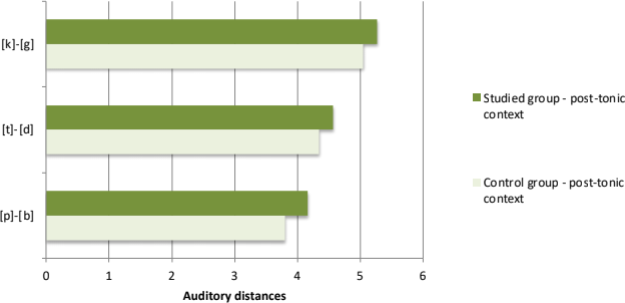
\includegraphics[width=\linewidth]{imgs/gregio-image14.png}
\caption{Auditory distances between voiceless and voiced pairs of speech productions in the post-tonic context of studied and control groups as a function of the judges' responses in the perception experiment.} 
\label{gregio-fig14}
\end{figure}



The logistic regression analysis revealed that the most influential acoustic
measures in the auditory judgments for the unvoiced plosive consonant were, in
the tonic context, duration of the previous vowel (V1) and f0 at the beginning
of the vowel (V2) (figure \ref{gregio-fig15}), and in the post-tonic context, duration of the
plosive consonant (C2) and f0 at the beginning of the vowel (V2) (figure \ref{gregio-fig16}).

\begin{figure}
\centering
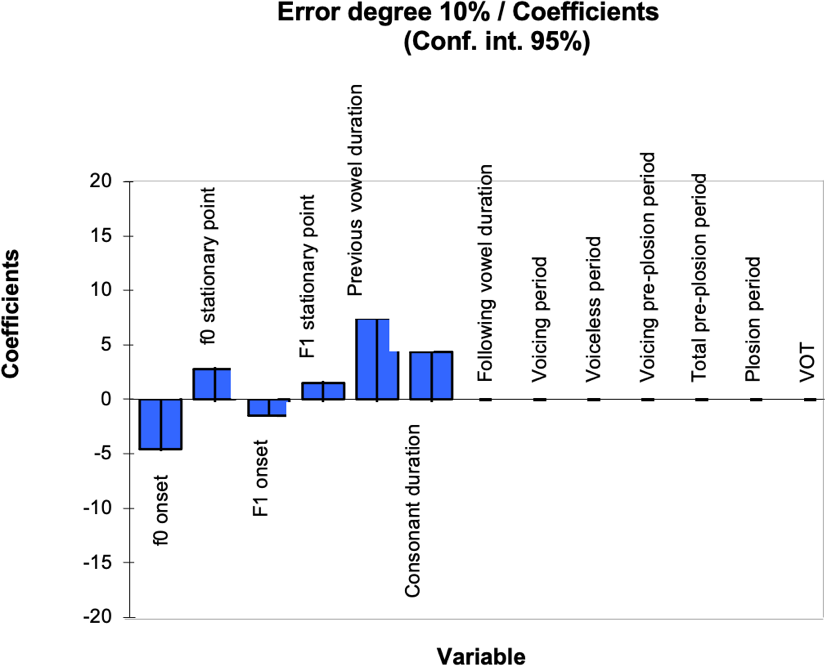
\includegraphics[width=0.9\linewidth]{imgs/gregio-image15.png}
\caption{Logistic regression analysis graph for the estimation of auditory judgments from the acoustic measures of the production of unvoiced plosive consonants in the tonic context by the studied and control groups.} 
\label{gregio-fig15}
\end{figure}

\begin{figure}
\centering
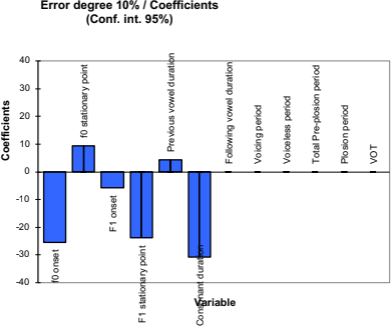
\includegraphics[width=0.9\linewidth]{imgs/gregio-image16.png}
\caption{Logistic regression analysis graph for the estimation of auditory judgments from the acoustic measures of the production of unvoiced plosive consonants in the post-tonic context by the studied and control groups.} 
\label{gregio-fig16}
\end{figure}

For the voiced plosive consonant, the most influential acoustic measures in the
auditory judgments were, in the tonic context, the duration of the plosive
consonant (C2), the duration of the total pre-plosion and the duration of the
voiceless period (figure \ref{gregio-fig17}), and in the post-tonic context, the duration of
the total pre-plosion period and duration of the voicing period (figure \ref{gregio-fig18}).

\begin{figure}
\centering
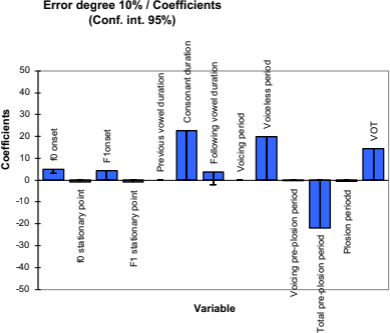
\includegraphics[width=0.9\linewidth]{imgs/gregio-image17.png}
\caption{Logistic regression analysis graph for the estimation of auditory judgments from the acoustic measures of the productions of voiced plosive consonants in the tonic context by the studied and control groups.} 
\label{gregio-fig17}
\end{figure}

\begin{figure}
\centering
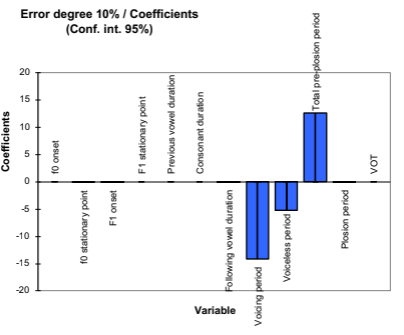
\includegraphics[width=0.9\linewidth]{imgs/gregio-image18.png}
\caption{Logistic regression analysis graph for the estimation of auditory judgments from the acoustic measures of voiced plosive consonant productions in the post-tonic context by the studied and control groups.} 
\label{gregio-fig18}
\end{figure}

The VOT duration measure was not revealed as a predictive acoustic cue in the
auditory judgment of voicing, in both stress contexts, while other duration
measures involved in the voicing bar details were deemed complementary in
explaining the implementations that speakers with disorders make and
influencing the perception of altered speech.

The data are corroborated by the BP studies that considered the gradient
productions from the voicing bar details in the productions of subjects with
hearing impairment \citep{ficker2003,barzaghi2007,pereira2012} and
without speech impairment \citep{gregio2011}, suggesting the relevance of
several acoustic cues for implementing voicing contrast.

In the voiced bilabial plosives of the studied group tonic context, a longer
period of voicing pre-plosion period was observed, suggesting an attempt to
guarantee the necessary voicing period, since bilabials, according to the
literature, have a longer voicing period. As for voiced plosive velar, no
voicing pre-plosion period was observed, suggesting that the speaker perceives
these differentiated cues for the articulatory points in trying to produce the
voicing contrast. The literature indicates that velar plosives have a shorter
duration of the voicing period \citep{van_alphen2004,lousada2005,barzaghi2007,pereira2012}.

As for the influence of the f0 at the beginning of the vowel, the voicing
contrast judgment revealed a predictive value with regard to unvoiced plosive
in both stress contexts. As the f0 measurement results from vocal fold
activity, which involves aerodynamic and physiological aspects, it tends to be
higher at the beginning of the vowel following an unvoiced consonant \citep{shimizu1996}.
The f0 measurement has been identified as an acoustic cue in voicing
contrasts \citep{whalen1993,hanson2009,gregio2011}. F1
measures, in turn, did not reveal a predictive value for the auditory judgment
of voicing in either stress context.

Regarding the duration measures of the V1C2V2 excerpt, the studied group
differentiated the duration of voiced and unvoiced segments, as it kept the
voiced plosive consonants’ duration shorter than the duration of their
respective unvoiced pairs, as expected based on the literature. However, the
studied group made this differentiation in a smaller proportion compared to the
control group, suggesting  difficulty in synchronizing the glottic and
supraglottic adjustments, given different timing of overlapping gestures. The
BP literature points to higher duration values for vowels preceding and
following consonants in the production of voiced plosive segments \citep{barbosa1996,gurgueira2006,britto2010},
justifying their influence on the auditory judgment of speech disorder.

As a final consideration, the acoustic measures that influenced the perception
of the auditory judgment of the voicing contrast have been shown to be
different for each stress context. The listener seems to attribute different
relevance to the acoustic cues involved in the auditory judgment of sound. The
perception of voicing contrasts showed that listeners integrate several
acoustic cues to identify and categorize a sound. Thus, a clinical diagnosis
based on only one acoustic measurement can be inaccurate.

Most of the speech samples from the studied group, who presented clinical
demand for speech therapy, could not be categorized as “sound exchanges or
absences” in view of the data exploration in this study. The subjects revealed
knowledge about the language, as they performed intermediate productions
towards the determinant characteristics of the voicing contrast. Such signs
denote that the subjects perceive differences and seek to implement different
actions to support the voicing contrast at different articulation points. The
acoustic cues relevant to the construction of voicing information resided in
parameters of duration, which suggest clues about the process of neuromotor
maturation of speech movements, aspects that have been suggested in previous
studies with children \citep{levy1993,Gama-Rossi,albano2007}.

The demand for temporal refinement surpassed the issues of implementation of
the f0 acoustic cue. Such aspects relate to the issue of synchronization of
glottic and supraglottic gestures, which is important for the construction of
voicing contrast information.

Thus, the exploration of the acoustic signal of the speech samples of the
studied group indicated an attempt to mark the voicing contrast, suggesting
that speakers perceive and try to differentiate in their production one sound
category from the other, yet these attempts are not always processed as
relevant information by the listener's perception.

Subjects control and organize their articulatory gestures in terms of physical
aspects and in terms of perceptual feedback (Gama-Rossi, 1999; Albano, 2001;
Albano, 2007). It is up to the professional to guide the child in their attempt
to achieve phonic contrast, producing articulatory targets that are audible to
the listener.

The challenge of working with issues that lie at the interface between speech
production and perception offers a rich field of reflection on the nature of
speech disorders. Such a challenge may result, in the future, in therapeutic
actions that consider the particularities of the manifestation in question,
which means contemplating the difficulties and recognizing the implementations
made by the speaker, which although not audible at first glance, can be
unveiled through instrumental investigation.

%%%%%%%%%%%%%%%%%%%%%%%%%%%%%%%%%%%%%%%%%%%%%%%%%%%%%%%%%%%%%%%%%%%%%%
\section{Conclusion}
The investigation showed evidence of more than one acoustic cue for the
implementation of voicing contrast. The duration of the plosive consonant,
voiceless period, and total pre-plosion period (tonic context) and the total
pre-plosion period and voicing period (post-tonic context) revealed predictive
power of the auditory judgment of the altered speech voicing contrast for
voiced plosives. For unvoiced plosive consonants, the influential measures were
f0 at the beginning of the vowel and duration of the previous vowel (tonic
context) and f0 at the beginning of the vowel and duration of the plosive
consonant (post-tonic context).


%%%%%%%%%%%%%%%%%%%%%%%%%%%%%%%%%%%%%%%%%%%%%%%%%%%%%%%%%%%%%%%%%%%%%%
\bibliographystyle{plainnat}
\bibliography{zuleicacamarg13.bib}
